\documentclass{standalone}

\usepackage{tikz}
\usepackage{amsmath, amssymb,stackrel}

%% Public TikZ libraries
\usetikzlibrary{arrows}
\usetikzlibrary{calc}
\usetikzlibrary{circuits.logic.US}
\usetikzlibrary{positioning}
\usetikzlibrary{shapes}

\DeclareMathOperator{\cor}{\mathbf{cor}}

%% Custom TikZ addons
	
%% Document

\begin{document}



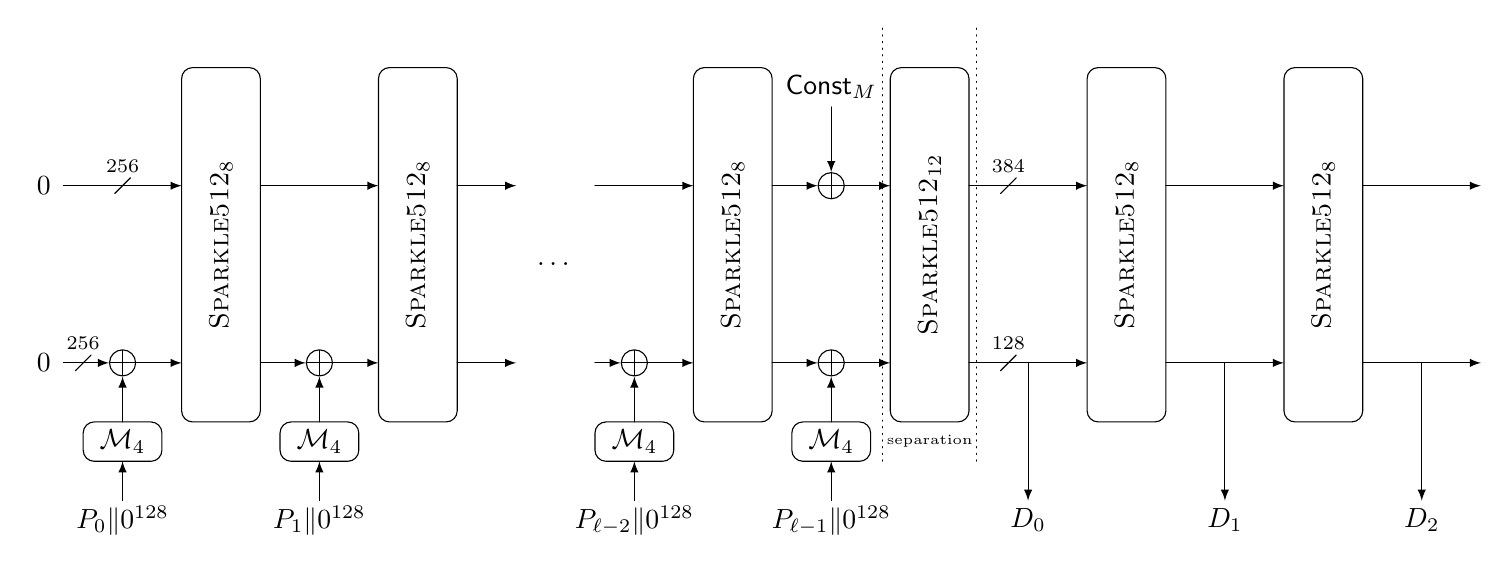
\begin{tikzpicture}[line cap=round]
\tikzset{tikzxor/.style={draw,circle,append after command={
        [shorten >=\pgflinewidth, shorten <=\pgflinewidth,]
        (\tikzlastnode.north) edge (\tikzlastnode.south)
        (\tikzlastnode.east) edge (\tikzlastnode.west)
        }
    }    
}

\tikzset{tikzadd/.style={draw,rectangle,append after command={
        [shorten >=\pgflinewidth, shorten <=\pgflinewidth,]
        (\tikzlastnode.north) edge (\tikzlastnode.south)
        (\tikzlastnode.east) edge (\tikzlastnode.west)
        }
    }   
}















\draw[rounded corners]  (-2.5,2.5) rectangle (-1.5,-2);
\draw[rounded corners]  (0,2.5) rectangle (1,-2);
\draw[rounded corners]  (4,2.5) rectangle (5,-2);
\draw[rounded corners]  (6.5,2.5) rectangle (7.5,-2);
\draw[rounded corners]  (9,2.5) rectangle (10,-2);
\draw[rounded corners]  (11.5,2.5) rectangle (12.5,-2);

\node[tikzxor] (v1) at (-3.25,-1.25) {};
\node[tikzxor] (v2) at (-0.75,-1.25) {};
\node[tikzxor] (v3) at (3.25,-1.25) {};
\node[tikzxor] (v4) at (5.75,-1.25) {};
\draw [-latex](-4,1) -- (-2.5,1);

\draw [-latex](-4,-1.25) -- (v1);
\draw [-latex](v1) -- (-2.5,-1.25);

\draw [-latex](-3.25,-2) -- (v1);

\draw [-latex](-1.5,-1.25) -- (v2);
\draw [-latex](v2) -- (-0,-1.25);
\draw [-latex](-1.5,1) -- (0,1);
\draw [-latex](-0.75,-2) -- (v2);
\draw [-latex](1,1) -- (1.75,1);
\draw [-latex](1,-1.25) -- (1.75,-1.25);
\node at (2.25,0) {$\dots$};
\draw [-latex](2.75,1) -- (4,1);
\draw [-latex](2.75,-1.25) -- (v3);
\draw [-latex](v3) -- (4,-1.25);
\draw [-latex](3.25,-2) -- (v3);
%\draw [-latex](5,1) -- (6.5,1);
\draw [-latex](5,-1.25) -- (v4);
\draw [-latex](v4) -- (6.5,-1.25);
\draw [-latex](5.75,-2) -- (v4);
\draw [-latex](7.5,1) -- (9,1);
\draw [-latex](10,1) -- (11.5,1);
\draw [-latex](7.5,-1.25) -- (9,-1.25);
\draw [-latex](10,-1.25) -- (11.5,-1.25);
\draw[dotted] (6.4,3) -- (6.4,-2.5);
\draw[dotted] (6.1+1.5,3) -- (6.1+1.5,-2.5);
\node at (7,-2.25) {\tiny separation};
\node[rotate=90] at (-2,0.25) {$\textsc{Sparkle512}_8$};
\node[rotate=90] at (0.5,0.25) {$\textsc{Sparkle512}_8$};
\node[rotate=90] at (4.5,0.25) {$\textsc{Sparkle512}_8$};
\node[rotate=90] at (7,0.25) {$\textsc{Sparkle512}_{12}$};
\node[rotate=90] at (9.5,0.25) {$\textsc{Sparkle512}_8$};

\node at (-4.25,-1.25) {$0$};
\node at (-4.25,1) {$0$};
\draw (-3.25-0.1,0.9) -- (-3.25+0.1,1.1);
\draw (-3.25-0.1+11.25,0.9) -- (-3.25+0.1+11.25,1.1);
\draw (-3.25-0.1-0.5,0.9-2.25) -- (-3.25+0.1-0.5,1.1-2.25);
\draw (-3.25-0.1-0.5+11.75,0.9-2.25) -- (-3.25+0.1-0.5+11.75,1.1-2.25);
\node at (-3.25,1.25) {\scriptsize $256$};
\node at (-3.75,-1) {\scriptsize $256$};
\node at (-3.25+11.25,1.25) {\scriptsize $384$};
\node at (-3.75+11.75,-1) {\scriptsize $128$};
\node at (-3.25,-3.25) {$P_0\|0^{128}$};
\node at (-0.75,-3.25) {$P_1\|0^{128}$};
\node at (3.25,-3.25) {$P_{\ell-2}\|0^{128}$};
\node at (5.75,-3.25) {$P_{\ell-1}\|0^{128}$};
\draw [-latex](8.25,-1.25) -- (8.25,-3);
\draw [-latex](10.75,-1.25) -- (10.75,-3);
\node at (8.25,-3.25) {$D_0$};
\node at (10.75,-3.25) {$D_1$};
\draw [-latex](12.5,1) -- (14,1);
\draw [-latex](12.5,-1.25) -- (14,-1.25);
\draw [-latex](13.25,-1.25) -- (13.25,-3);
\node at (13.25,-3.25) {$D_2$};
\node[rotate=90] at (12,0.25) {$\textsc{Sparkle512}_8$};
\node[tikzxor] (v5) at (5.75,1) {};
\draw [-latex](5,1) -- (v5);
\draw [-latex](v5) -- (6.5,1);
\draw [-latex](5.75,2) -- (v5);
\node at (5.75,2.25) {$\mathsf{Const}_M$};
\draw[rounded corners]  (5.25,-2) rectangle (6.25,-2.5);
\draw[rounded corners]  (2.75,-2) rectangle (3.75,-2.5);
\draw[rounded corners]  (-1.25,-2) rectangle (-0.25,-2.5);
\draw[rounded corners]  (-3.75,-2) rectangle (-2.75,-2.5);


\draw[-latex] (5.75,-3) -- (5.75,-2.5);
\draw[-latex] (3.25,-3) -- (3.25,-2.5);
\draw[-latex] (-0.75,-3) -- (-0.75,-2.5);
\draw[-latex] (-3.25,-3) -- (-3.25,-2.5);
\node at (-3.25,-2.25) {$\mathcal{M}_4$};
\node at (-0.75,-2.25) {$\mathcal{M}_4$};
\node at (3.25,-2.25) {$\mathcal{M}_4$};
\node at (5.75,-2.25) {$\mathcal{M}_4$};
\end{tikzpicture}
\end{document}
